\section{Motivation and Challenges}
\label{sec:motivation}

Kernel tuning is crucial to system performance, yet difficult in practice. To understand what matters, we conducted a large-scale empirical study over 1{,}000 workload--hardware pairs (CPU-bound, memory-intensive analytics, I/O-intensive streaming, sensor, HPC, ML inference, real-time audio, and more); the six workloads used for controlled evaluation (see \emph{Setup}) are drawn from this study, and the full pair-level dataset is released in our anonymized artifact. In each we varied dozens of settings and measured median and 95\% tail latency, throughput, anomaly rate, and fairness.

\paragraph{Observation~1 -- Context Sensitivity.} Optimal values vary widely across workloads and even across phases of one workload. Shrinking \texttt{sched\_latency\_ns} improved tail latency by 21\% for web-serving but caused a 20\% fairness drop under mixed streaming; adjusting reclamation knobs (\texttt{vm.swappiness}, \texttt{dirty\_ratio}) boosted steady-state throughput but degraded responsiveness during bursty loads. Similar context-dependence appeared across CPU scheduling, interrupt routing, and NUMA placement.

\paragraph{Observation~2 -- Strong inter-parameter dependencies.}
% --- Added: Pairwise Effects figure (single column) ---
\begin{figure}[t]
 \centering
 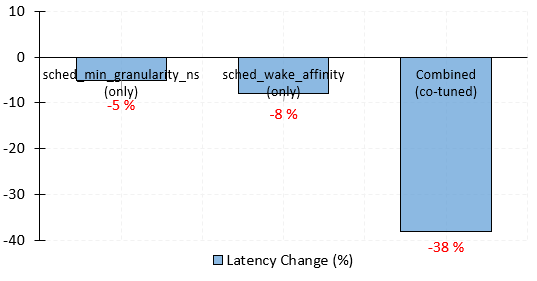
\includegraphics[width=0.74\linewidth]{figures/pairwise_effects.png}
 \caption{\textbf{Effect on Kernel Tunable Parameter Pairs.}
 Tuning \texttt{sched\_wake\_affinity} and \texttt{sched\_min\_granularity\_ns} simultaneously has a nonlinear synergistic effect on reducing tail latency, indicating that these parameters are strongly linked to each other and cannot be tuned independently.}
 \label{fig:pairwise}
\end{figure}


As shown in Figure~\ref{fig:pairwise}, these \emph{advanced interactions} are better resolved by collaborative tuning than by modifying parameters individually. Contrary to the common belief that parameters can be tuned independently, changing either \texttt{sched\_min\_granularity\_ns} or \texttt{sched\_wake\_affinity} in isolation produced little improvement, yet modifying both simultaneously reduced tail latency by more than 30\%. A similar nonlinear synergy emerged between CPU scheduling and memory reclamation: settings suboptimal in isolation became overall-optimal when combined with complementary settings.

\paragraph{Observation~3 -- Trade-offs between competing objectives.} Improving one dimension often harms others: reducing latency frequently increased starvation, and maximizing throughput could degrade fairness, especially under contention or NUMA imbalance---and more so as resources saturate. A practical solution must therefore model trade-offs explicitly and explain them, so operators can choose among Pareto-optimal configurations by objective.

\paragraph{Summary of findings.} Kernel tuning is characterized by (i)~context-dependence, (ii)~coupled inter-parameter effects, and (iii)~multi-objective trade-offs---explaining why static and black-box techniques struggle in practice. SemantOS addresses these with segmented telemetry, a semantic knowledge base that captures and analyzes parameter interactions, and multi-objective decision-making.